% -*- root: warwickthesis.tex -*-

\chapter{RNA-seq pre-processing}
\label{cha:mcf10a-results}
\label{sec:sequencing-depth-rna}

\begin{figure}[!h]
  \centering
  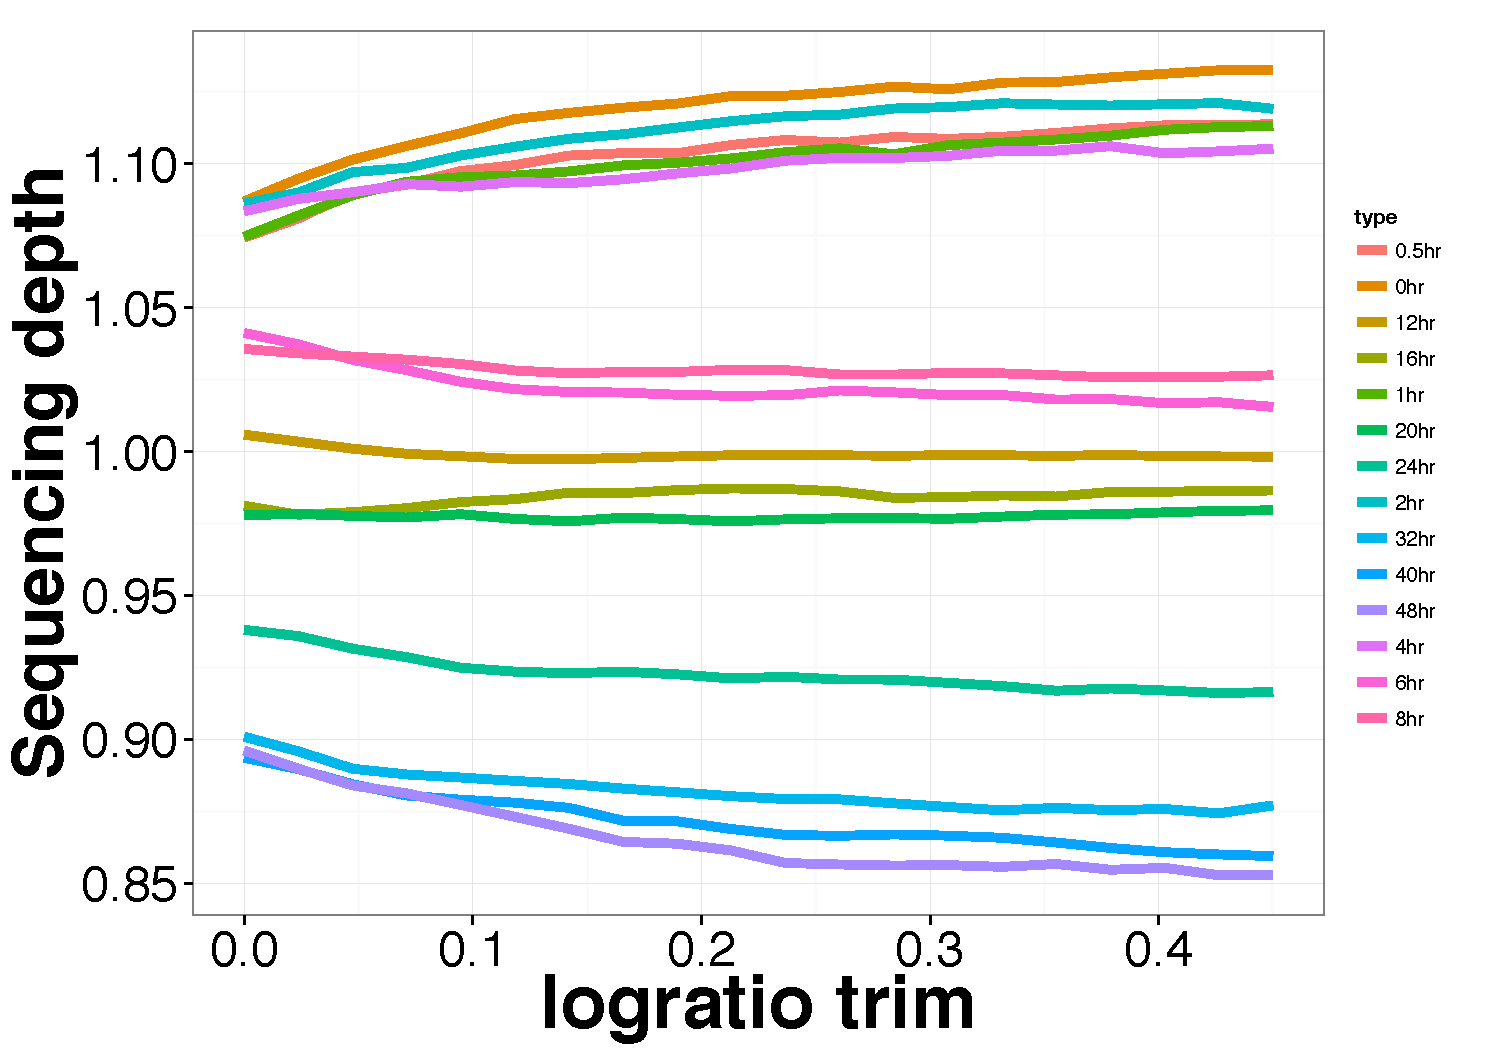
\includegraphics[width=0.8\textwidth]{pics/sequencing-depth.pdf}
  \caption{To determine sequencing depth from RNA-seq experiments we pre-process data using the \emph{edgeR} package. See package \cite{Robinson:2010cw} for details of exact usage which briefly outlined in Section \ref{sec:normalisation}. We propose a strategy of trimming the $\log$ ratio eqn. (\ref{eq:MA-values}) at different values and identifying the cutoff that stabilises sequencing depths for the different samples. For this example we chose $0.4$.}
  \label{fig:seq-depth}
\end{figure}

\newgeometry{left=2.45cm, top=3cm}
\definecolor{NavyBlue}{RGB}{35,96,184}
\definecolor{MidnightBlue}{RGB}{11, 83, 130}
\rowcolors{2}{NavyBlue!30}{white}
\begin{table}[ht]
\begin{tabular}{l|ccccccc}
  \hline
\rowcolor{MidnightBlue!50}
& 0hr & 0.5hr & 1hr & 2hr & 4hr & 6hr & 8hr \\
  \hline
MFGE8 & 62.35 & 47.88 & 63.05 & 53.02 & 46.26 & 35.66 & 46.50 \\
  MFGE8 raw count & 916.00 & 874.00 & 1046.00 & 774.00 & 708.00 & 496.00 & 654.00 \\
  CCDC99 & 64.19 & 78.61 & 65.76 & 67.81 & 78.86 & 78.23 & 59.65 \\
  CCDC99 raw count & 943.00 & 1435.00 & 1091.00 & 990.00 & 1207.00 & 1088.00 & 839.00 \\
  TAB2 & 96.59 & 117.40 & 105.66 & 98.64 & 91.80 & 95.85 & 108.64 \\
  TAB2 raw count & 1419.00 & 2143.00 & 1753.00 & 1440.00 & 1405.00 & 1333.00 & 1528.00 \\
  ZSWIM6 & 19.13 & 19.12 & 18.93 & 20.07 & 16.66 & 21.79 & 24.25 \\
  ZSWIM6 raw count & 281.00 & 349.00 & 314.00 & 293.00 & 255.00 & 303.00 & 341.00 \\
  FLRT3 & 18.18 & 22.95 & 17.42 & 14.86 & 24.18 & 47.53 & 53.47 \\
  FLRT3 raw count & 267.00 & 419.00 & 289.00 & 217.00 & 370.00 & 661.00 & 752.00 \\
  HTRA1 & 231.45 & 211.19 & 193.78 & 205.63 & 207.32 & 166.74 & 159.48 \\
  HTRA1 raw count & 3400.00 & 3855.00 & 3215.00 & 3002.00 & 3173.00 & 2319.00 & 2243.00 \\
  NCOA4 & 232.13 & 238.91 & 171.78 & 238.10 & 268.28 & 261.94 & 214.94 \\
  NCOA4 raw count & 3410.00 & 4361.00 & 2850.00 & 3476.00 & 4106.00 & 3643.00 & 3023.00 \\
  TGIF1 & 39.75 & 42.51 & 47.68 & 40.55 & 41.29 & 50.40 & 47.21 \\
  TGIF1 raw count & 584.00 & 776.00 & 791.00 & 592.00 & 632.00 & 701.00 & 664.00 \\
  IL1RAP & 94.48 & 90.83 & 81.37 & 90.76 & 153.22 & 416.82 & 422.42 \\
  IL1RAP raw count & 1388.00 & 1658.00 & 1350.00 & 1325.00 & 2345.00 & 5797.00 & 5941.00 \\
  CSRNP1 & 19.20 & 17.37 & 37.55 & 84.80 & 16.14 & 40.48 & 53.04 \\
  CSRNP1 raw count & 282.00 & 317.00 & 623.00 & 1238.00 & 247.00 & 563.00 & 746.00 \\
  SEPT9 & 337.84 & 352.21 & 392.74 & 348.45 & 359.88 & 572.56 & 647.45 \\
  SEPT9 raw count & 4963.00 & 6429.00 & 6516.00 & 5087.00 & 5508.00 & 7963.00 & 9106.00 \\
  SF3A3 & 133.83 & 155.20 & 113.37 & 133.43 & 146.49 & 148.48 & 136.66 \\
  SF3A3 raw count & 1966.00 & 2833.00 & 1881.00 & 1948.00 & 2242.00 & 2065.00 & 1922.00 \\
  ESR1 & 1184.12 & 1258.93 & 2332.92 & 1103.56 & 845.35 & 470.68 & 618.94 \\
  ESR1 raw count & 17395.00 & 22980.00 & 38706.00 & 16111.00 & 12938.00 & 6546.00 & 8705.00 \\
  C1orf43 & 382.43 & 383.05 & 282.08 & 368.72 & 344.20 & 306.09 & 299.69 \\
  C1orf43 raw count & 5618.00 & 6992.00 & 4680.00 & 5383.00 & 5268.00 & 4257.00 & 4215.00 \\
  STMN1 & 365.96 & 368.80 & 279.54 & 336.12 & 329.89 & 290.49 & 249.28 \\
  STMN1 raw count & 5376.00 & 6732.00 & 4638.00 & 4907.00 & 5049.00 & 4040.00 & 3506.00 \\
  PFDN5 & 153.57 & 116.20 & 91.80 & 103.84 & 116.69 & 110.37 & 104.09 \\
  PFDN5 raw count & 2256.00 & 2121.00 & 1523.00 & 1516.00 & 1786.00 & 1535.00 & 1464.00 \\
  LDHB & 1280.10 & 1252.25 & 913.31 & 1167.27 & 1225.75 & 1222.57 & 1129.88 \\
  LDHB raw count & 18805.00 & 22858.00 & 15153.00 & 17041.00 & 18760.00 & 17003.00 & 15891.00 \\
  XPO6 & 169.98 & 187.91 & 205.65 & 182.34 & 172.10 & 216.50 & 218.50 \\
  XPO6 raw count & 2497.00 & 3430.00 & 3412.00 & 2662.00 & 2634.00 & 3011.00 & 3073.00 \\
  RPS25 & 402.65 & 299.45 & 228.43 & 279.13 & 287.16 & 282.79 & 269.83 \\
  RPS25 raw count & 5915.00 & 5466.00 & 3790.00 & 4075.00 & 4395.00 & 3933.00 & 3795.00 \\
  DYSF & 2.04 & 2.08 & 1.27 & 1.16 & 1.05 & 1.87 & 3.06 \\
  DYSF raw count & 30.00 & 38.00 & 21.00 & 17.00 & 16.00 & 26.00 & 43.00 \\
   \hline
\end{tabular}
\caption{The table shows a very small sample of data used in Chapter \protect\ref{cha:oncog-transf} and we show the effect on the data due to normalisation, see Section \protect\ref{sec:technique-bio} for details of the normalisation. The white rows show data after normalisation and the blue rows the corresponding raw counts obtained from RNA-seq}
\label{tab:norm-mcf10a}
\end{table}
\restoregeometry

%%% Local Variables:
%%% TeX-master: "warwickthesis"
%%% End:
